Implementada a solução, foram construídas algumas cenas
tridimensionais que pretendem testar a funcionalidade
da solução obtida.
\newline
\break
\noindent
Estas cenas pretendem demonstrar o uso de transformações
e sub-grupos de forma a construir figuras reconhecíveis.
\newline
\break
\noindent
Estas cenas podem, então, ser observados nas figuras
\ref{fig:snowman}, \ref{fig:solarlign} e \ref{fig:solar}.

\subsection{Boneco de Neve}

\begin{center}
    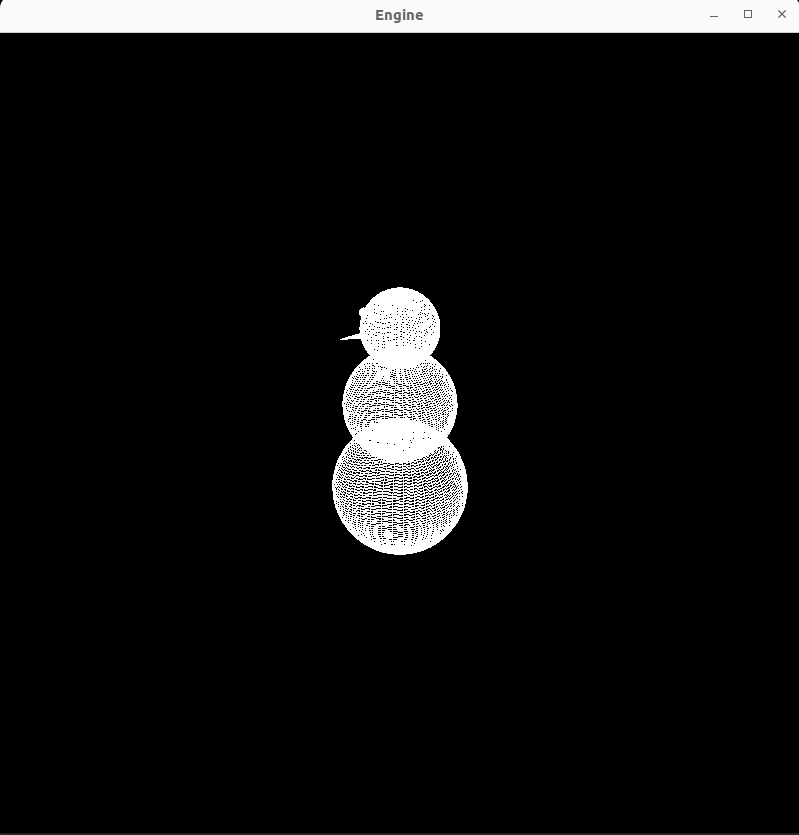
\includegraphics[width=0.8\textwidth]{imgs/boneconeve.png}
    \captionof{figure}{Boneco de Neve construído com transformações}
    \label{fig:snowman}
\end{center}

\subsection{Sistema Solar Alinhado}

\begin{center}
    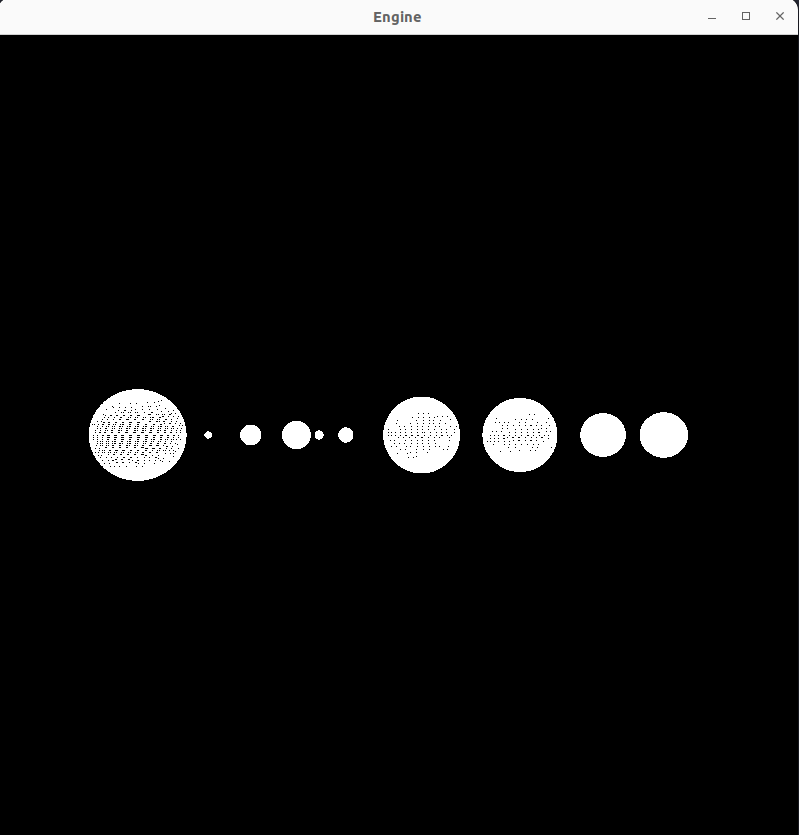
\includegraphics[width=0.8\textwidth]{imgs/sissolarhor.png}
    \captionof{figure}{Sistema Solar construído com transformações}
    \label{fig:solarlign}
\end{center}

\subsection{Sistema Solar}

\begin{center}
    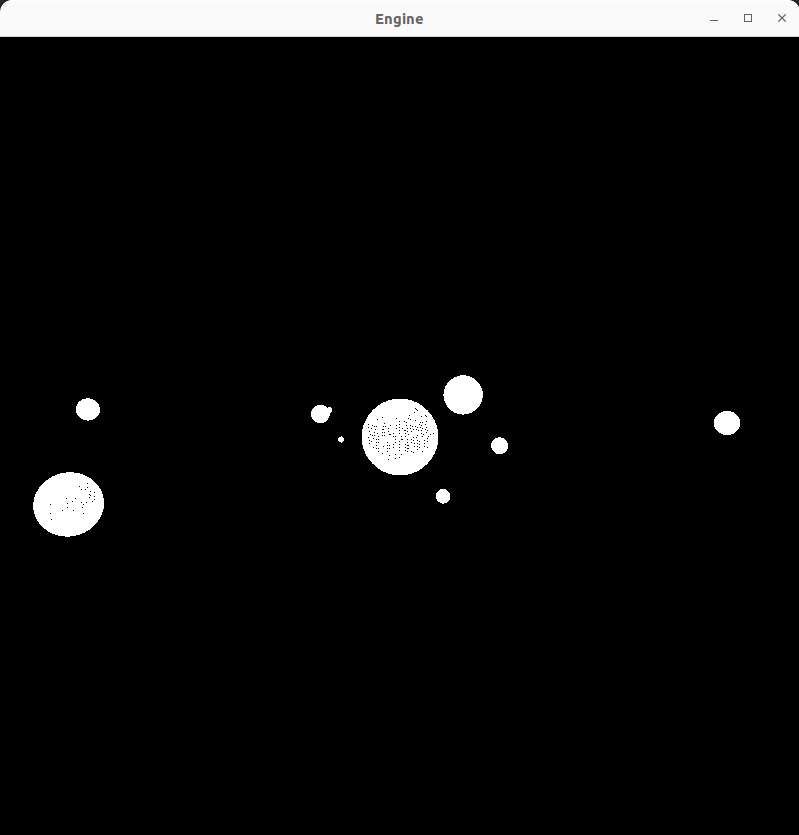
\includegraphics[width=0.8\textwidth]{imgs/sissolar.png}
    \captionof{figure}{Sistema Solar disperso construído com transformações}
    \label{fig:solar}
\end{center}

